\section*{SHAP}

The use of SHAP values is a simple method to measure the impact of features on any model. Intuitively, it consists in adding/removing a feature and measure the impact of the removal on the prediction. Thus, it aims at finding \textit{marginal} contributions of features. 

The concept of SHAP is based on Lloyd Shapley's results on game theory. Shapley's main idea is that members should receive payments proportional to their marginal contributions to the society. 

\textit{Note}: the explanation of the game theory part is based on \href{https://www.youtube.com/watch?v=qcLZMYPdpH4}{Stanford tutorial}.

The main question is: what weighting system should we use? \\

Let $N$ be a coalition with all members involved, and $S$ a coalition with any member(s).

$v$ is the value brought to the society by a specific coalition. \\

Shapley considers several axioms: \\

\textbf{Symmetry}: for all $S$ that contains neither $i$ nor $j$, $i$ and $j$ are interchangeable if $v(S \cup \{i\})=v(S \cup \{j\})$. Then interchangeable agents should receive the same payments: $\phi_i(N,v)=\phi_j(N,v)$.

Intuitively, agents who contribute the same should receive the same payments. \\

\textbf{Dummy players}: $i$ is a dummy player if the amount that $i$ contributes to any coalition is $0$: for all $S$, $v(S \cup \{i\})=v(S)$. Then for any $v$, if $i$ is a dummy player: $\phi_i(N,v)=0$.

Intuitively, dummy players should receive nothing. \\

\textbf{Additivity}: if we can separate a game in two parts: $v=v_1 + v_2$, then we should be able to decompose the payments: $\phi_i(N, v_1+v_2) = \phi_i(N, v_1) + \phi_i(N, v_2)$.

For instance, we can consider a game that consists in producing fruits during two days. An agent will receive equally the fruits production of day 1 and day 2 than receiving the total production for these two days. \\

Based on the previous axioms, it turns out that there is only one way of defining the payment of each agent:

$$\phi_i(N, v) = \frac{1}{|N|!} \Sigma_{S \subseteq N\setminus \{i\}} |S|! (|N| - |S| - 1)! (v({S \cup \{i\}}) - v(S))$$

Warning: here $|.|$ is the \textit{cardinality} of a set (not the absolute value function!) \\

$v({S \cup \{i\}}) - v(S)$ is the marginal contribution of agent $i$.

The rest of the formula consists in weighting the marginal contribution with all possible coalitions. More specifically:

$|S|!$ is the number of times $S$ could have been formed.

$(|N| - |S| - 1)!$ is the number of times the remaining agents could have been added.

$\frac{1}{|N|!}$ is used to average across all different possible coalitions. \\

The next part of this section is inspired by a \href{https://towardsdatascience.com/shap-explained-the-way-i-wish-someone-explained-it-to-me-ab81cc69ef30?}{very good tutorial} on how the Shapley value is applied to machine learning. \\

Here, the "game" is what produces the outcome of a model. The "agents" or "players" are the features of the model. \\

Let's consider a model that consists in predicting the income of an individual based on the age, the gender and the job.

To define all the possible coalitions, we use the mathematical concept \textit{power set}:

\begin{center}
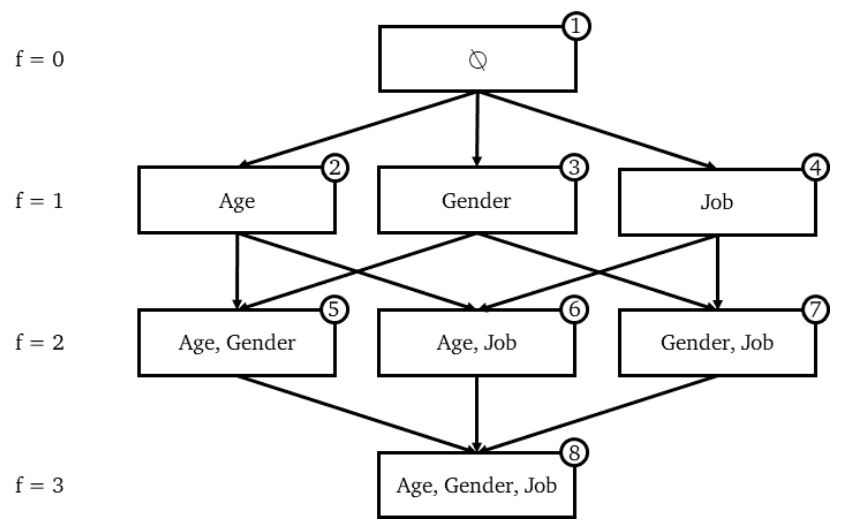
\includegraphics[scale=0.35]{powerset_1.png}
\end{center}

Once the training is done, we compute the prediction for each coalition:

\begin{center}
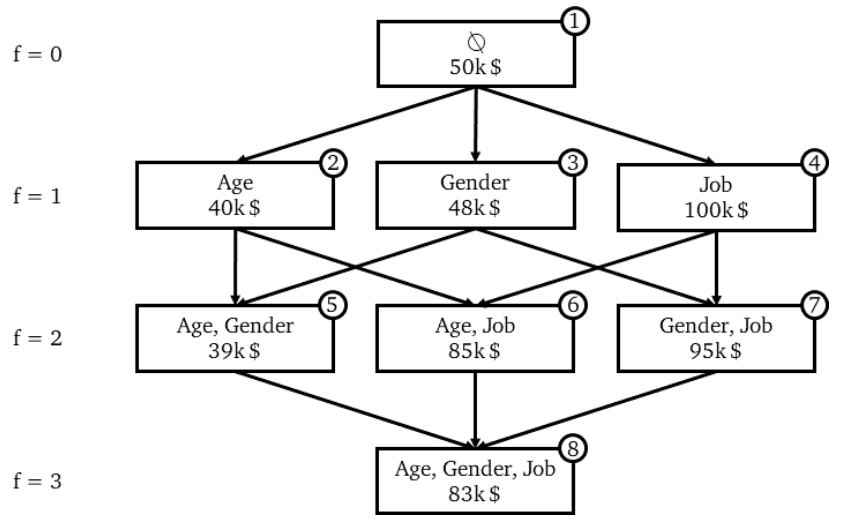
\includegraphics[scale=0.35]{powerset_2.png}
\end{center}

We note that an edge (or an arrow) is the effect of a marginal contribution. \\

With machine learning notation, the marginal contribution is:

$$MC_{feat 1, \{feat 1, feat 2\}} = Predict_{feat 1, feat 2}(X) - Predict_{feat 2}(X)$$

\textit{Note}: for classification problems that output probabilities, the marginal contribution is the difference in probabilities for each class. The final output of SHAP is split by classes:.

\begin{center}
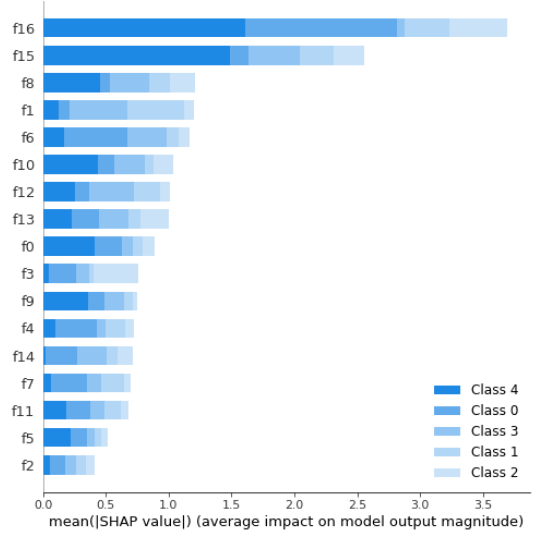
\includegraphics[scale=0.30]{shap_classification.png}
\end{center}

$MC_{feat 1, \{feat 1, feat 2\}}$ should be read: "the effect of feature 1 in coalition \{feat 1, feat 2\}".

In the above example, $MC_{Age, \{Age\}} (X) = 40k\$ - 50k\$ = -10k\$$. \\

The SHAP value is defined as such:

\begin{align*}
  SHAP_{Age}(X) &= \omega_1 MC_{Age, \{Age\}}(X)  \\
            &= + \omega_2 MC_{Age, \{Age, Gender\}}(X)  \\
	   &= + \omega_3 MC_{Age, \{Age, Job\}}(X) \\
	   &= + \omega_4 MC_{Age, \{Age, Gender, Job\}}(X)
\end{align*}

Under the constraint: $\omega_1 + \omega_2 + \omega_3 + \omega_4 = 1$ \\

Thus, the SHAP value is the average of all impacts a feature brings to every coalition. \\

But how to find the weights? \\

The weights are based on the number of edges for the specific level of the power set we are looking at. Mathematically, it's the inverse of the function $f*C_f^F$. For example, for the level $f=2$, $\omega_3 = \frac{1}{2*C_2^3} = \frac{1}{6}$. \\

Warning: if feature 1 contributes more than feature 2, it doesn't mean that feature 1 improves more the model than feature 2! As mentioned by the \href{https://github.com/slundberg/shap/issues/367}{author}, "SHAP values of a model's output explain how features impact the output of the model, not if that impact is good or bad".\\

One of the main limits of SHAP is that it has a lot to compute. \textbf{The cardinality of a power set is $2^n$.} This is thus the number of model to train (with the same parameters and input data) to compute the Shapley value ($n$ = number of features = $F$ in our case). Fortunately, the method used approximation without computing all possible cases. \\

\vspace{5mm}